\documentclass[11pt]{article}

\usepackage{fullpage}
\usepackage{amsmath}
\usepackage{epsfig}
\usepackage{graphics}
\usepackage{caption}
\usepackage{circuitikz}

\oddsidemargin -0.15in
\evensidemargin -0.15in
\headheight 0in
\headsep 0in
%\topmargin -0.25in
\textheight 9.3in
\textwidth 6.8in

\begin{document}


\begin{center}
\section*{
Franklin \& Marshall College \hfill PHY 223\\
\bigskip
{\Large \it Photoelectric effect}}
\end{center}

The emission and absorption of light was an early subject for investigation by
German physicist Max Planck. As Planck attempted to formulate a theory to
explain the spectral distribution of emitted light based on a classical wave
model, he ran into considerable difficulty. Classical theory (Rayleigh-Jeans
law) predicted that the amount of light emitted from a hot, glowing body (a
black body) would increase dramatically as the wavelength decreased, whereas
experiment showed that it approached zero. This discrepancy became known as the
ultraviolet catastrophe. Experimental data for the radiation of light by a black
body showed a distribution having a peak at a wavelength inversely proportional
to temperature (Wien’s law). The classical prediction for the distribution had
no maximum at all. In order to reconcile theory with laboratory results, Planck
was forced to develop a new model for light called the quantum model. In this
model, light is emitted in small, discrete bundles or quanta.

\vspace{5mm}

\noindent {\bf Theoretical background}

\vspace{3mm}

\begin{center}
{\it Planck's quantum theory}
\end{center}

By the late 1800's many physicists thought that they had explained all the main
principles of the universe and discovered all the natural laws. But as
scientists continued working, inconsistencies that couldn't easily be explained
began showing up in some areas of study.

In 1901 Planck published his law of radiation. In it he stated that an
oscillator, or any similar physical system, has a discrete set of possible
energy values or levels; energies between these values never occur. Planck went
on to state that the emission and absorption of radiation is associated with the
transitions or jumps between two energy levels. The energy lost or gained by the
oscillator is emitted or absorbed as a quantum of radiant energy, the magnitude
of which is expressed by the equation:

\begin{equation}
E = hf
\end{equation}

\noindent where E equals the radiant energy, f is the frequency of the
radiation, and h is a fundamental constant of nature. The constant, h , became
known as Planck's constant. Planck's constant was found to have significance
beyond relating the frequency and energy of light, and became a cornerstone of
the quantum mechanical view of the subatomic world. In 1918, Planck was awarded
a Nobel prize for introducing the quantum of light.

\vspace{3mm}

\begin{center}
{\it The Photoelectric effect}
\end{center}

In photoelectric emission, light strikes a material, causing electrons to be
emitted. The classical wave model predicted that as the intensity of incident
light was increased, the amplitude and thus the energy of the wave would
increase. This would then cause more energetic photoelectrons to be emitted. The
new quantum model, however, predicted that higher frequency light would produce
higher energy photoelectrons, independent of intensity, while increased
intensity would only increase the number of electrons emitted (or photoelectric
current). In the early 1900s several investigators found that the kinetic energy
of the photoelectrons was dependent on the wavelength, or frequency, and
independent of intensity, while the magnitude of the photoelectric current, or
number of electrons was dependent on the intensity as predicted by the quantum
model. Einstein applied Planck's theory and explained the photoelectric effect
in terms of the quantum model using his famous equation for which he received
the Nobel prize in 1921:

\begin{equation}
E = hf = KE_{max} + W_0
\end{equation}

\noindent where KE max is the maximum kinetic energy of the emitted
photoelectrons, and W 0 is the energy needed to remove them from the surface of
the material (the work function). E is the energy supplied by the quantum of
light known as a photon.

\vspace{3mm}

\begin{center}
{\it The h/e experiment}
\end{center}

A light photon with energy hf is incident upon an electron in a cathode of a
vacuum tube. The electron uses a minimum W 0 of its energy to escape the cathode,
leaving it with a maximum energy of KE max in the form of kinetic energy. Normally the
emitted electrons reach the anode of the tube, and can be measured as a photoelectric
current. However, by applying a reverse potential V between the anode and the cathode,
the photoelectric current can be stopped. KE max can be determined my measuring the
minimum reverse potential needed to stop the photoelectrons and reduce the photoelectric
current to zero (but see Note 1). Relating kinetic energy to stopping potential gives the
equation:

\begin{equation}
  KE_{max} = eV
\end{equation}

Therefore, using Einstein's equation,

\begin{equation}
  hf = eV + W_0
\end{equation}

When solved for V, the equation becomes:

\begin{equation}
  V = (h/e)f - (W_0/e)
\end{equation}

If we plot $V$ as a function of $f$ for different frequencies of light, the $V$
intercept is equal to $-W_0/e$ and the slope is $h/e$. Coupling our experimental
determination of the ratio $h/e$ with the accepted value for $e$, $1.602 \times
10^{-19}$ C, we can determine Planck's constant, $h$.

\vspace{5mm}

\noindent {\bf Experimental setup}

Set up the equipment as shown in Fig \ref{fig exp setup}. Focus the light from
the Mercury Vapor Light Source onto the slot in the white reflective mask on the
h /e Apparatus. Tilt the Light Shield of the Apparatus out of the way to reveal
the white photodiode mask inside the Apparatus (see Fig \ref{fig detector}).
Slide the Lens/Grating assembly forward and back on its support rods until you
achieve the sharpest image of the aperture centered on the hole in the
photodiode mask. Secure the Lens/Grating by tightening the thumbscrew.

\vspace{3mm}

\begin{minipage}{\linewidth}
  \centering
  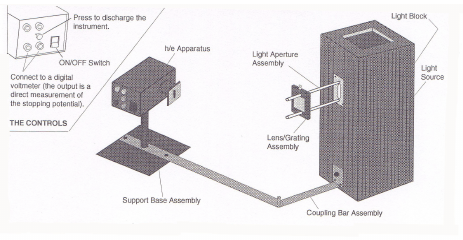
\includegraphics[scale=3.0]{./Experimental_setup.png}
  \captionof{figure}{Photoelectric effect experimental setup}
  \label{fig exp setup}
\end{minipage}

\vspace{3mm}

Align the system by rotating the h/e Apparatus on its support base so that the
same color light that falls on the opening of the light screen falls on the
window in the photodiode mask with no overlap of color from the other spectral
bands. Return the Light Shield to its closed position.

\vspace{3mm}

\begin{minipage}{\linewidth}
  \centering
  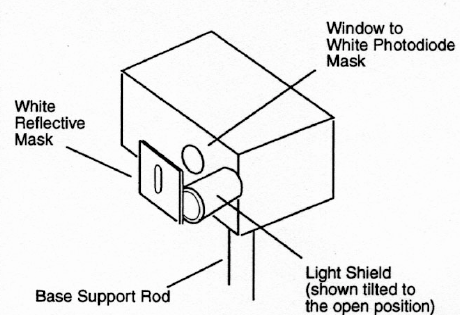
\includegraphics[scale=2.0]{./Detector.png}
  \captionof{figure}{Detail of photodiode housing}
  \label{fig detector}
\end{minipage}

\vspace{3mm}

Check the polarity of the leads from your digital voltmeter (DVM), and connect
them to the OUTPUT terminals of the same polarity on the h /e Apparatus.

The h/e Apparatus includes two filters: one Green, and one Yellow. The filter
frames have magnetic strips and mount to the outside of the White Reflective
mask of the h /e Apparatus. Use the green and yellow filters when you're using
the green and yellow spectral lines. These filters limit higher frequencies of
light from entering the h /e Apparatus. This prevents ambient room light from
interfering with the lower energy yellow and green light and masking the true
results. It also blocks the higher frequency ultraviolet light from the higher
order spectra which may overlap with lower orders of yellow and green.

Instead of applying a reverse voltage manually to find the stopping potential
(when the current stops), we let the freed electrons accumulate across the face
of a capacitor. This generates a reverse potential. When enough charges have
accumulated, the voltage across the capacitor prevents charges from moving
across the gap and the voltage stabilizes. A button on the side of the detector
can discharge the capacitor, allowing charges to flow again.

\vspace{5mm}

\noindent {\bf Procedure}

\begin{enumerate}

\item Turn the mercury lamp on. It might take a few seconds to light up.
  
\item You can see five colors in two orders of the mercury light spectrum (see
Fig \ref{fig lines}). Adjust the h /e Apparatus carefully so that only one color
from the first order (the brightest order) falls on the opening of the mask of
the photodiode. You will need to open the light shield (as in Fig \ref{fig
detector}) in order to see the photodiode. Close the light shield when the
apparatus is adjusted for the particular wavelength that you are using.

\vspace{3mm}

\begin{minipage}{\linewidth}
  \centering
  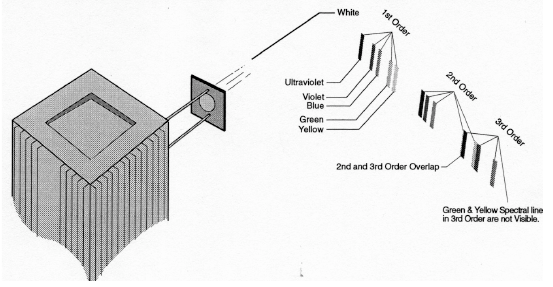
\includegraphics[scale=2.0]{./Spectral_lines.png}
  \captionof{figure}{The Mercury lamp spectrum}
  \label{fig lines}
\end{minipage}

\vspace{3mm}

\item For each color in the first order, measure the stopping potential with the
multimeter and record that measurement in a table. Before reading the
multimeter, press the "PUSH TO ZERO" button on the side panel of the h/e
Apparatus to discharge any accumulated potential in the unit's electronics. This
will assure the Apparatus records only the potential of the light you are
measuring. (Note that the output voltage will drift with the absence of light on
the photodiode.) Use the yellow and green colored filters on the Reflective Mask
of the h/e Apparatus when you measure the yellow and green spectral lines.

\item Find uncertainties in your stopping potentials by repeating the
measurement of each several times. Consider also the intrinsic uncertainty due
to the multimeter itself.

\item Move to the second order and repeat the process. Record your results.
 
\end{enumerate}

\vspace{5mm}

\noindent {\bf Analysis}

\begin{enumerate}

\item Determine the wavelength and frequency of each spectral line. Plot a graph
of the stopping potential vs. frequency. Make separate plots for your first
order measurements and your second order measurements.

\item Determine the slope and y-intercept. Interpret the results in terms of the
h/e ratio and the $W_0/e$ ratio. Calculate h and $W_0$.

\item In your discussion, report your values and discuss your results with an
interpretation based on a quantum model of light.
\end{enumerate}

\vspace{3mm}

\begin{center}
  {\it The mercury spectrum}
\end{center}

\begin{center}
\begin{tabular}{l c}
  Color & Wavelength (nm) \\
  Yellow & 578.0 \\
  Green & 546.1 \\
  Blue & 435.8 \\
  Violet & 404.7 \\
  Ultraviolet & 365.5 \\
\end{tabular}
\end{center}

\end{document}